% Options for packages loaded elsewhere
\PassOptionsToPackage{unicode}{hyperref}
\PassOptionsToPackage{hyphens}{url}
%
\documentclass[
]{book}
\usepackage{amsmath,amssymb}
\usepackage{iftex}
\ifPDFTeX
  \usepackage[T1]{fontenc}
  \usepackage[utf8]{inputenc}
  \usepackage{textcomp} % provide euro and other symbols
\else % if luatex or xetex
  \usepackage{unicode-math} % this also loads fontspec
  \defaultfontfeatures{Scale=MatchLowercase}
  \defaultfontfeatures[\rmfamily]{Ligatures=TeX,Scale=1}
\fi
\usepackage{lmodern}
\ifPDFTeX\else
  % xetex/luatex font selection
\fi
% Use upquote if available, for straight quotes in verbatim environments
\IfFileExists{upquote.sty}{\usepackage{upquote}}{}
\IfFileExists{microtype.sty}{% use microtype if available
  \usepackage[]{microtype}
  \UseMicrotypeSet[protrusion]{basicmath} % disable protrusion for tt fonts
}{}
\makeatletter
\@ifundefined{KOMAClassName}{% if non-KOMA class
  \IfFileExists{parskip.sty}{%
    \usepackage{parskip}
  }{% else
    \setlength{\parindent}{0pt}
    \setlength{\parskip}{6pt plus 2pt minus 1pt}}
}{% if KOMA class
  \KOMAoptions{parskip=half}}
\makeatother
\usepackage{xcolor}
\usepackage{color}
\usepackage{fancyvrb}
\newcommand{\VerbBar}{|}
\newcommand{\VERB}{\Verb[commandchars=\\\{\}]}
\DefineVerbatimEnvironment{Highlighting}{Verbatim}{commandchars=\\\{\}}
% Add ',fontsize=\small' for more characters per line
\usepackage{framed}
\definecolor{shadecolor}{RGB}{248,248,248}
\newenvironment{Shaded}{\begin{snugshade}}{\end{snugshade}}
\newcommand{\AlertTok}[1]{\textcolor[rgb]{0.94,0.16,0.16}{#1}}
\newcommand{\AnnotationTok}[1]{\textcolor[rgb]{0.56,0.35,0.01}{\textbf{\textit{#1}}}}
\newcommand{\AttributeTok}[1]{\textcolor[rgb]{0.13,0.29,0.53}{#1}}
\newcommand{\BaseNTok}[1]{\textcolor[rgb]{0.00,0.00,0.81}{#1}}
\newcommand{\BuiltInTok}[1]{#1}
\newcommand{\CharTok}[1]{\textcolor[rgb]{0.31,0.60,0.02}{#1}}
\newcommand{\CommentTok}[1]{\textcolor[rgb]{0.56,0.35,0.01}{\textit{#1}}}
\newcommand{\CommentVarTok}[1]{\textcolor[rgb]{0.56,0.35,0.01}{\textbf{\textit{#1}}}}
\newcommand{\ConstantTok}[1]{\textcolor[rgb]{0.56,0.35,0.01}{#1}}
\newcommand{\ControlFlowTok}[1]{\textcolor[rgb]{0.13,0.29,0.53}{\textbf{#1}}}
\newcommand{\DataTypeTok}[1]{\textcolor[rgb]{0.13,0.29,0.53}{#1}}
\newcommand{\DecValTok}[1]{\textcolor[rgb]{0.00,0.00,0.81}{#1}}
\newcommand{\DocumentationTok}[1]{\textcolor[rgb]{0.56,0.35,0.01}{\textbf{\textit{#1}}}}
\newcommand{\ErrorTok}[1]{\textcolor[rgb]{0.64,0.00,0.00}{\textbf{#1}}}
\newcommand{\ExtensionTok}[1]{#1}
\newcommand{\FloatTok}[1]{\textcolor[rgb]{0.00,0.00,0.81}{#1}}
\newcommand{\FunctionTok}[1]{\textcolor[rgb]{0.13,0.29,0.53}{\textbf{#1}}}
\newcommand{\ImportTok}[1]{#1}
\newcommand{\InformationTok}[1]{\textcolor[rgb]{0.56,0.35,0.01}{\textbf{\textit{#1}}}}
\newcommand{\KeywordTok}[1]{\textcolor[rgb]{0.13,0.29,0.53}{\textbf{#1}}}
\newcommand{\NormalTok}[1]{#1}
\newcommand{\OperatorTok}[1]{\textcolor[rgb]{0.81,0.36,0.00}{\textbf{#1}}}
\newcommand{\OtherTok}[1]{\textcolor[rgb]{0.56,0.35,0.01}{#1}}
\newcommand{\PreprocessorTok}[1]{\textcolor[rgb]{0.56,0.35,0.01}{\textit{#1}}}
\newcommand{\RegionMarkerTok}[1]{#1}
\newcommand{\SpecialCharTok}[1]{\textcolor[rgb]{0.81,0.36,0.00}{\textbf{#1}}}
\newcommand{\SpecialStringTok}[1]{\textcolor[rgb]{0.31,0.60,0.02}{#1}}
\newcommand{\StringTok}[1]{\textcolor[rgb]{0.31,0.60,0.02}{#1}}
\newcommand{\VariableTok}[1]{\textcolor[rgb]{0.00,0.00,0.00}{#1}}
\newcommand{\VerbatimStringTok}[1]{\textcolor[rgb]{0.31,0.60,0.02}{#1}}
\newcommand{\WarningTok}[1]{\textcolor[rgb]{0.56,0.35,0.01}{\textbf{\textit{#1}}}}
\usepackage{longtable,booktabs,array}
\usepackage{calc} % for calculating minipage widths
% Correct order of tables after \paragraph or \subparagraph
\usepackage{etoolbox}
\makeatletter
\patchcmd\longtable{\par}{\if@noskipsec\mbox{}\fi\par}{}{}
\makeatother
% Allow footnotes in longtable head/foot
\IfFileExists{footnotehyper.sty}{\usepackage{footnotehyper}}{\usepackage{footnote}}
\makesavenoteenv{longtable}
\usepackage{graphicx}
\makeatletter
\newsavebox\pandoc@box
\newcommand*\pandocbounded[1]{% scales image to fit in text height/width
  \sbox\pandoc@box{#1}%
  \Gscale@div\@tempa{\textheight}{\dimexpr\ht\pandoc@box+\dp\pandoc@box\relax}%
  \Gscale@div\@tempb{\linewidth}{\wd\pandoc@box}%
  \ifdim\@tempb\p@<\@tempa\p@\let\@tempa\@tempb\fi% select the smaller of both
  \ifdim\@tempa\p@<\p@\scalebox{\@tempa}{\usebox\pandoc@box}%
  \else\usebox{\pandoc@box}%
  \fi%
}
% Set default figure placement to htbp
\def\fps@figure{htbp}
\makeatother
\setlength{\emergencystretch}{3em} % prevent overfull lines
\providecommand{\tightlist}{%
  \setlength{\itemsep}{0pt}\setlength{\parskip}{0pt}}
\setcounter{secnumdepth}{5}
\usepackage[]{natbib}
\bibliographystyle{plainnat}
\usepackage{bookmark}
\IfFileExists{xurl.sty}{\usepackage{xurl}}{} % add URL line breaks if available
\urlstyle{same}
\hypersetup{
  pdftitle={Machine Learning for Biostatistics},
  pdfauthor={Armando Teixeira-Pinto},
  hidelinks,
  pdfcreator={LaTeX via pandoc}}

\title{Machine Learning for Biostatistics}
\usepackage{etoolbox}
\makeatletter
\providecommand{\subtitle}[1]{% add subtitle to \maketitle
  \apptocmd{\@title}{\par {\large #1 \par}}{}{}
}
\makeatother
\subtitle{Module 3}
\author{Armando Teixeira-Pinto}
\date{2025-07-18}

\begin{document}
\maketitle

{
\setcounter{tocdepth}{1}
\tableofcontents
}
\chapter*{Resampling methods}\label{resampling-methods}
\addcontentsline{toc}{chapter}{Resampling methods}

\section*{Introduction}\label{introduction}
\addcontentsline{toc}{section}{Introduction}

This module will cover \textbf{bootstrap} and \textbf{cross-validation}. These are two
important techniques that are useful to study sample variability, evaluate
model performance and choosing \emph{tuning} parameters in many of the methods
covered in this unit.

We will switch the order presented in the book \emph{Introduction to Statistical
Learning} and start with bootstrap and then proceed to cross-validation.

By the end of this module you should be able to:

\begin{enumerate}
\def\labelenumi{\arabic{enumi}.}
\tightlist
\item
  Be able to compute standard errors for different statistics
  through bootstrapping
\item
  Compute model performance statistics by cross-validation
\item
  Use cross-validation to select \emph{tuning} parameters such
  as the number of neighbours in KNN
\end{enumerate}

\section*{Dataset used in the examples}\label{dataset-used-in-the-examples}
\addcontentsline{toc}{section}{Dataset used in the examples}

The file \href{https://www.dropbox.com/s/7wjsfdaf0wt2kg2/bmd.csv?dl=1}{bmd.csv}
contains 169 records of bone densitometries (measurement of
bone mineral density). The following variables were collected:

\begin{itemize}
\tightlist
\item
  id -- patient's number
\item
  age -- patient's age
\item
  fracture -- hip fracture (fracture / no fracture)
\item
  weight\_kg -- weight measured in Kg
\item
  height\_cm -- height measure in cm
\item
  waiting\_time -- time the patient had to wait for the densitometry (in minutes)
\item
  bmd -- bone mineral density measure in the hip
\end{itemize}

\begin{center}\rule{0.5\linewidth}{0.5pt}\end{center}

The file \href{https://www.dropbox.com/s/wg32uj43fsy9yvd/SBI.csv?dl=0}{SBI.csv}
contains the records of 2349 children admitted to the
emergency room with fever and tested for serious bacterial infection (sbi).
The following variables were collected:

\begin{itemize}
\tightlist
\item
  id -- patient's number
\item
  fever\_hours -- duration of the fever in hours
\item
  age -- child's age
\item
  sex -- child's sex (M / F)
\item
  wcc -- white cell count
\item
  prevAB -- previous antibiotics (Yes / No)
\item
  sbi -- serious bacterial infection (Not Applicable / UTI / Pneum / Bact)
\item
  pct -- procalcitonin
\item
  crp -- c-reactive protein
\end{itemize}

\begin{center}\rule{0.5\linewidth}{0.5pt}\end{center}

\section*{Slides}\label{slides}
\addcontentsline{toc}{section}{Slides}

You can download the slides used in the videos for resampling methods:

\begin{itemize}
\tightlist
\item
  \href{https://www.dropbox.com/s/wbwlcxwxnyf4bvi/Module-3-Resampling-methods_2020.pdf?dl=0}{Slides}
\end{itemize}

\chapter{Bootstrap}\label{bootstrap}

\section{Introduction}\label{boot.intro}

Bootstrap was proposed by
\href{https://projecteuclid.org/download/pdf_1/euclid.aos/1176344552}{Efron in 1979}
and it mimics the sampling process by sampling with replacement
the original sample. This process replicates the sample variation and allows
the calculation of standard errors. It can also be used to refine more
complex machine learning algorithms, as we will see later.

From the original sample of size \(n\), we create many (e.g.~10,000) samples of
size \(n\) by sampling from the original sample with replacement. Notice that the replacement
allows the same value to be included multiple times in the same sample. This
is why you can create many different samples.
For each of the bootstrapped samples we compute the statistics of interest. The
standard deviation of all these computed statistics, is the standard error.

\section{Readings}\label{boot.read}

Read the following chapter of \emph{An introduction to statistical learning}:

\begin{itemize}
\tightlist
\item
  5.2 The Bootstrap
\end{itemize}

\section{Practice session}\label{boot.prac}

\subsection*{Task - Confidence intervals with bootstrap}\label{task---confidence-intervals-with-bootstrap}
\addcontentsline{toc}{subsection}{Task - Confidence intervals with bootstrap}

We will be using the
\href{https://www.dropbox.com/s/7wjsfdaf0wt2kg2/bmd.csv?dl=1}{bmd.csv}
dataset to plot the histogram, compute the median and 95\% confidence interval
for the ``waiting\_time''

Let's first read the data and create the variable BMI that will be used later.

\begin{Shaded}
\begin{Highlighting}[]
\FunctionTok{library}\NormalTok{(caret) }\CommentTok{\#library for Machine Learning}
\end{Highlighting}
\end{Shaded}

\begin{verbatim}
## Warning: package 'ggplot2' was built under R version 4.3.3
\end{verbatim}

\begin{Shaded}
\begin{Highlighting}[]
\FunctionTok{library}\NormalTok{(boot)  }\CommentTok{\#library for bootstrap}
\FunctionTok{library}\NormalTok{(pROC)  }\CommentTok{\#library for the ROC curve}
\FunctionTok{library}\NormalTok{(Rmisc) }\CommentTok{\#CI() function to compute conf interval}
\FunctionTok{set.seed}\NormalTok{(}\DecValTok{1974}\NormalTok{)}

\CommentTok{\#the option stringsAsFactors = TRUE in the command below converts }
\CommentTok{\#string variables as sex into factor variables}
\NormalTok{bmd.data }\OtherTok{\textless{}{-}} \FunctionTok{read.csv}\NormalTok{(}\StringTok{"https://www.dropbox.com/s/c6mhgatkotuze8o/bmd.csv?dl=1"}\NormalTok{, }
                     \AttributeTok{stringsAsFactors =} \ConstantTok{TRUE}\NormalTok{)}
\CommentTok{\#computes the BMI}
\NormalTok{bmd.data}\SpecialCharTok{$}\NormalTok{bmi }\OtherTok{\textless{}{-}}\NormalTok{ bmd.data}\SpecialCharTok{$}\NormalTok{weight\_kg }\SpecialCharTok{/}\NormalTok{ (bmd.data}\SpecialCharTok{$}\NormalTok{height\_cm}\SpecialCharTok{/}\DecValTok{100}\NormalTok{)}\SpecialCharTok{\^{}}\DecValTok{2}
\end{Highlighting}
\end{Shaded}

Let's plot the histogram for \emph{waiting time} and compute the median

\begin{Shaded}
\begin{Highlighting}[]
\FunctionTok{hist}\NormalTok{(bmd.data}\SpecialCharTok{$}\NormalTok{waiting\_time)}
\end{Highlighting}
\end{Shaded}

\pandocbounded{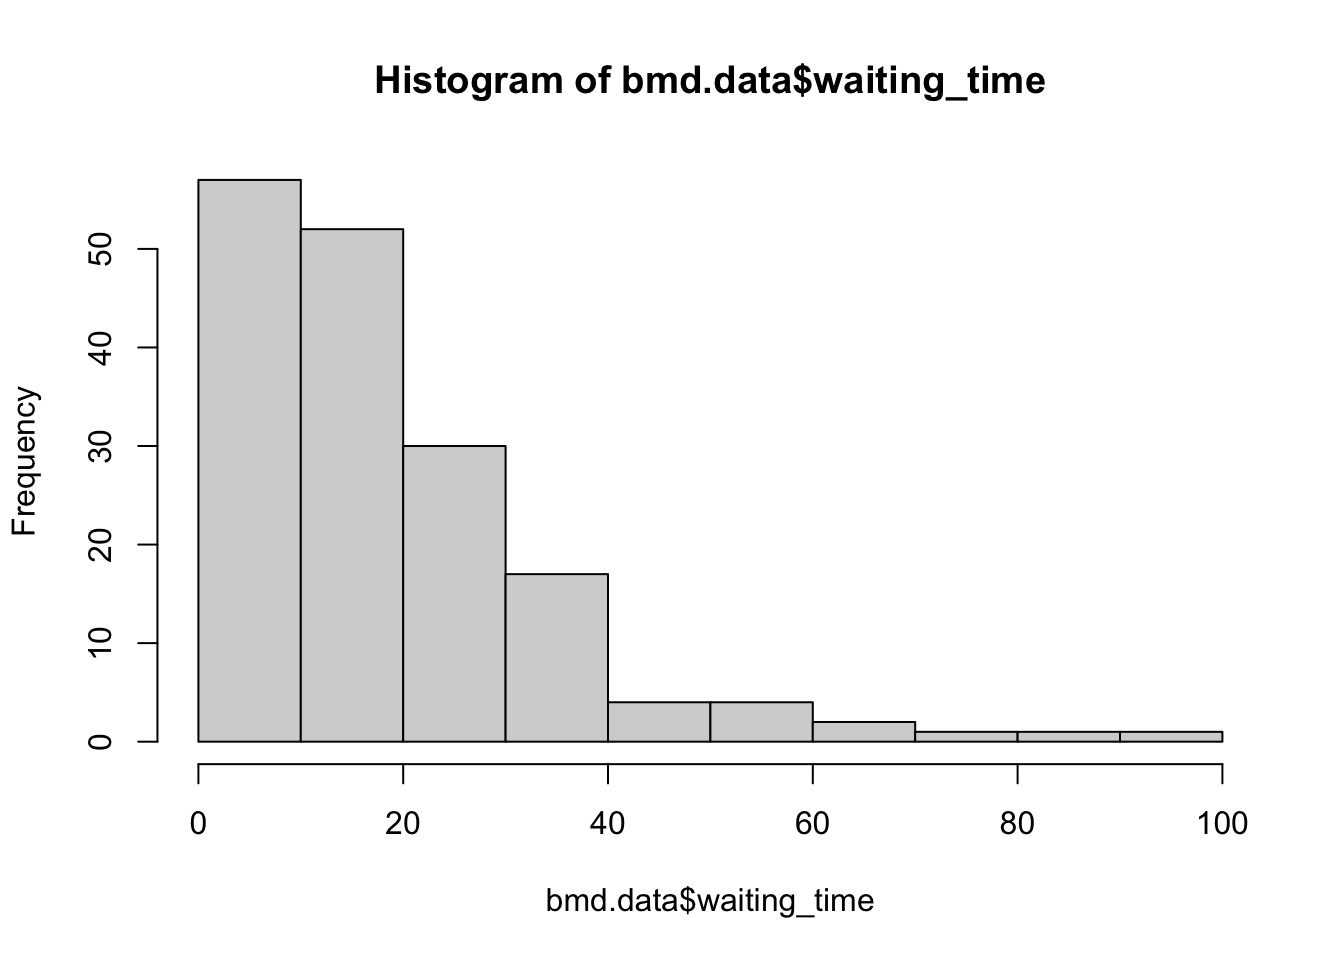
\includegraphics[keepaspectratio]{_main_files/figure-latex/unnamed-chunk-2-1.pdf}}

\begin{Shaded}
\begin{Highlighting}[]
\FunctionTok{median}\NormalTok{(bmd.data}\SpecialCharTok{$}\NormalTok{waiting\_time)}
\end{Highlighting}
\end{Shaded}

\begin{verbatim}
## [1] 14
\end{verbatim}

And now use the function \textbf{boot()}, from the library \textbf{boot}, to bootstrap the median. We will also compute it manually

\begin{Shaded}
\begin{Highlighting}[]
\CommentTok{\#using the boot function}
\FunctionTok{median}\NormalTok{(bmd.data}\SpecialCharTok{$}\NormalTok{waiting\_time)}
\end{Highlighting}
\end{Shaded}

\begin{verbatim}
## [1] 14
\end{verbatim}

\begin{Shaded}
\begin{Highlighting}[]
\NormalTok{samplemedian }\OtherTok{\textless{}{-}} \ControlFlowTok{function}\NormalTok{(x, d) \{ }\CommentTok{\#need to define the function to use bootstrap}
  \FunctionTok{return}\NormalTok{(}\FunctionTok{median}\NormalTok{(x[d]))           }\CommentTok{\#d is the index for the bootstrap}
\NormalTok{\}}
\NormalTok{bootresults }\OtherTok{\textless{}{-}} \FunctionTok{boot}\NormalTok{(bmd.data}\SpecialCharTok{$}\NormalTok{waiting\_time, }\AttributeTok{statistic=}\NormalTok{samplemedian, }\AttributeTok{R=}\DecValTok{10000}\NormalTok{)}
\CommentTok{\# get 95\% confidence interval }
\FunctionTok{boot.ci}\NormalTok{(bootresults, }\AttributeTok{type=}\StringTok{"perc"}\NormalTok{)}
\end{Highlighting}
\end{Shaded}

\begin{verbatim}
## BOOTSTRAP CONFIDENCE INTERVAL CALCULATIONS
## Based on 10000 bootstrap replicates
## 
## CALL : 
## boot.ci(boot.out = bootresults, type = "perc")
## 
## Intervals : 
## Level     Percentile     
## 95%   (13, 18 )  
## Calculations and Intervals on Original Scale
\end{verbatim}

\begin{Shaded}
\begin{Highlighting}[]
\CommentTok{\#manual bootstrap}
\NormalTok{median.bs }\OtherTok{\textless{}{-}} \ConstantTok{NA}
\ControlFlowTok{for}\NormalTok{ (i }\ControlFlowTok{in} \DecValTok{1}\SpecialCharTok{:}\DecValTok{10000}\NormalTok{)\{ }\CommentTok{\# change to 10000}
\NormalTok{  sample.bs    }\OtherTok{\textless{}{-}} \FunctionTok{sample}\NormalTok{(bmd.data}\SpecialCharTok{$}\NormalTok{waiting\_time, }\DecValTok{169}\NormalTok{, }\AttributeTok{replace =} \ConstantTok{TRUE}\NormalTok{)}
\NormalTok{  median.bs[i] }\OtherTok{\textless{}{-}} \FunctionTok{median}\NormalTok{(sample.bs)}
\NormalTok{\}}
\FunctionTok{median}\NormalTok{(median.bs)  }\CommentTok{\#median (could use mean) of all the bootstrapped medians}
\end{Highlighting}
\end{Shaded}

\begin{verbatim}
## [1] 14
\end{verbatim}

\begin{Shaded}
\begin{Highlighting}[]
\FunctionTok{sd}\NormalTok{(median.bs)      }\CommentTok{\#Std error of the median}
\end{Highlighting}
\end{Shaded}

\begin{verbatim}
## [1] 1.34752
\end{verbatim}

\begin{Shaded}
\begin{Highlighting}[]
\FunctionTok{quantile}\NormalTok{(median.bs, }\FunctionTok{c}\NormalTok{(}\FloatTok{0.025}\NormalTok{, }\FloatTok{0.975}\NormalTok{))  }\CommentTok{\#95\% empirical confidence interval}
\end{Highlighting}
\end{Shaded}

\begin{verbatim}
##  2.5% 97.5% 
##    12    18
\end{verbatim}

\textbf{TRY IT YOURSELF:}

\begin{enumerate}
\def\labelenumi{\arabic{enumi})}
\tightlist
\item
  Compute the mean for \emph{waiting\_time} and the usual 95\% confidence
  interval using the \textbf{CI()} function.
\end{enumerate}

\emph{See the solution code}

\begin{Shaded}
\begin{Highlighting}[]
\CommentTok{\#library(Rmisc) \#CI() function to compute the conf interval for the mean}
\FunctionTok{CI}\NormalTok{(bmd.data}\SpecialCharTok{$}\NormalTok{waiting\_time)}
\end{Highlighting}
\end{Shaded}

\begin{enumerate}
\def\labelenumi{\arabic{enumi})}
\setcounter{enumi}{1}
\tightlist
\item
  Compute the 95\% confidence interval for the mean using the boot function
\end{enumerate}

\emph{See the solution code}

\begin{Shaded}
\begin{Highlighting}[]
\FunctionTok{CI}\NormalTok{(bmd.data}\SpecialCharTok{$}\NormalTok{waiting\_time)}

\NormalTok{samplemean }\OtherTok{\textless{}{-}} \ControlFlowTok{function}\NormalTok{(x, d) \{ }\CommentTok{\#need to define the function to use bootstrap}
  \FunctionTok{return}\NormalTok{(}\FunctionTok{mean}\NormalTok{(x[d]))           }\CommentTok{\#d is the index for the bootstrap}
\NormalTok{\}}

\NormalTok{bootresults }\OtherTok{\textless{}{-}} \FunctionTok{boot}\NormalTok{(bmd.data}\SpecialCharTok{$}\NormalTok{waiting\_time, }\AttributeTok{statistic=}\NormalTok{samplemean, }\AttributeTok{R=}\DecValTok{10000}\NormalTok{)}
\FunctionTok{boot.ci}\NormalTok{(bootresults, }\AttributeTok{type=}\StringTok{"perc"}\NormalTok{)}
\end{Highlighting}
\end{Shaded}

\section{Exercises}\label{boot.exerc}

Solve the following exercises:

The \href{https://www.dropbox.com/s/4t7nph5d97hq0qh/diabetes.csv?dl=1}{diabetes data}
were provided by Hastie and Tibshirani (1990, p.~6).
The observations arise from a study of the factors affecting patterns of
insulin-dependent diabetes mellitus in 43 children (Sockett et al., 1987).
The aim was to investigate the dependence of serum C-peptide on other factors,
better to understand the patterns of residual insulin secretion.

The response, \emph{cpep}, is the log of C-peptide concentration at diagnosis, and
the selected covariates are \emph{age}, the child's age at diagnosis, and \emph{base},
minus their base deficit. Base deficit is a measure of acidity.

\begin{enumerate}
\def\labelenumi{\arabic{enumi})}
\item
  Calculate the Pearson correlation coefficient between \emph{cpep} and \emph{base} with
  the respective 95\% confidence interval obtained by the \href{https://en.wikipedia.org/wiki/Fisher_transformation}{Fisher's
  z-transformation} (the
  usual way of getting the confidence interval for the Pearson's correlation)\\
  \emph{Note: you can use the function CIr in the ``psychometric'' package}
\item
  Write your own function to compute the 95\% confidence interval
  for the above correlation, using bootstrap.
\item
  Use the function \emph{boot()} from the \emph{boot} package to compute
  the 95\% confidence interval through bootstrap
\item
  Plot the histogram with the correlations obtained in
  the bootstrap samples.
\end{enumerate}

\emph{See the solution code}

\begin{Shaded}
\begin{Highlighting}[]
\CommentTok{\#install.packages("psychometric") \# install package with function for}
                                 \CommentTok{\# the correlation confidence interval}
\CommentTok{\#install.packages("boot")         \# install package for bootstrap function}
\FunctionTok{library}\NormalTok{(boot)}
\FunctionTok{library}\NormalTok{(psychometric) }
\end{Highlighting}
\end{Shaded}

\begin{verbatim}
## Warning: package 'dplyr' was built under R version 4.3.1
\end{verbatim}

\begin{verbatim}
## Warning: package 'purrr' was built under R version 4.3.3
\end{verbatim}

\begin{Shaded}
\begin{Highlighting}[]
\FunctionTok{set.seed}\NormalTok{(}\DecValTok{1001}\NormalTok{)}
\NormalTok{myData }\OtherTok{\textless{}{-}} \FunctionTok{read.csv}\NormalTok{(}\StringTok{"https://www.dropbox.com/s/6rc00ealjtyp3qi/diabetes.csv?dl=1"}\NormalTok{)}

\NormalTok{sample.size }\OtherTok{\textless{}{-}} \FunctionTok{dim}\NormalTok{(myData)[}\DecValTok{1}\NormalTok{] }\CommentTok{\#nr of observations}

\CommentTok{\#1 {-} the Person correlation}
  \FunctionTok{cor}\NormalTok{(myData}\SpecialCharTok{$}\NormalTok{base, myData}\SpecialCharTok{$}\NormalTok{cpep)}
  \FunctionTok{CIr}\NormalTok{( }\AttributeTok{r =} \FunctionTok{cor}\NormalTok{(myData}\SpecialCharTok{$}\NormalTok{base, myData}\SpecialCharTok{$}\NormalTok{cpep),   }\CommentTok{\#conf interval using}
       \AttributeTok{n =}\NormalTok{ sample.size, }\AttributeTok{level =}\NormalTok{ .}\DecValTok{95}\NormalTok{)        }\CommentTok{\# Fisher\textquotesingle{}s z{-}transformations}

\CommentTok{\#2 {-} Bootstrap}
\NormalTok{  n.boot   }\OtherTok{\textless{}{-}} \DecValTok{25000}  \CommentTok{\#choose how many bootstraps}
\NormalTok{  cor.boot }\OtherTok{\textless{}{-}} \ConstantTok{NULL} \CommentTok{\# to store the bootstrap correlations}
  
  \CommentTok{\#manually implementing bootstrap}
  \ControlFlowTok{for}\NormalTok{ (i }\ControlFlowTok{in} \DecValTok{1}\SpecialCharTok{:}\NormalTok{n.boot) \{}
\NormalTok{    id.bs }\OtherTok{\textless{}{-}} \FunctionTok{sample.int}\NormalTok{(sample.size,   }\CommentTok{\#bootstrap the}
\NormalTok{                        sample.size,   }\CommentTok{\#original sample}
                        \AttributeTok{replace =} \ConstantTok{TRUE}\NormalTok{)}
\NormalTok{    cor.boot[i] }\OtherTok{\textless{}{-}} \FunctionTok{cor}\NormalTok{(myData[id.bs, ])[}\DecValTok{2}\NormalTok{,}\DecValTok{3}\NormalTok{]  }\CommentTok{\#Compute correlation}
                                              \CommentTok{\#between}
\NormalTok{   \}}
   \FunctionTok{quantile}\NormalTok{(cor.boot, }\FunctionTok{c}\NormalTok{(}\FloatTok{0.025}\NormalTok{, }\FloatTok{0.975}\NormalTok{))  }\CommentTok{\#95\% confidence interval}
  
\CommentTok{\#3 {-} Using the boot() function}
\NormalTok{  sample.corr }\OtherTok{\textless{}{-}} \ControlFlowTok{function}\NormalTok{(data, d) \{  }
    \FunctionTok{return}\NormalTok{(}\FunctionTok{cor}\NormalTok{(data}\SpecialCharTok{$}\NormalTok{base[d], data}\SpecialCharTok{$}\NormalTok{cpep[d]))   }\CommentTok{\#d is the index for the bootstrap}
\NormalTok{  \}}
    
\NormalTok{  bootcorr }\OtherTok{\textless{}{-}} \FunctionTok{boot}\NormalTok{(myData, }
                   \AttributeTok{statistic=}\NormalTok{sample.corr, }
                   \AttributeTok{R=}\NormalTok{n.boot)}
  \CommentTok{\# get 95\% confidence interval }
  \FunctionTok{boot.ci}\NormalTok{(bootcorr, }\AttributeTok{type=}\StringTok{"perc"}\NormalTok{)}

\CommentTok{\#4 {-} Histogram}
  \CommentTok{\#the correlations for the bootstrap samples}
  \CommentTok{\#are stored in bootcorr$t}
  \FunctionTok{hist}\NormalTok{(bootcorr}\SpecialCharTok{$}\NormalTok{t)}
\end{Highlighting}
\end{Shaded}

\pandocbounded{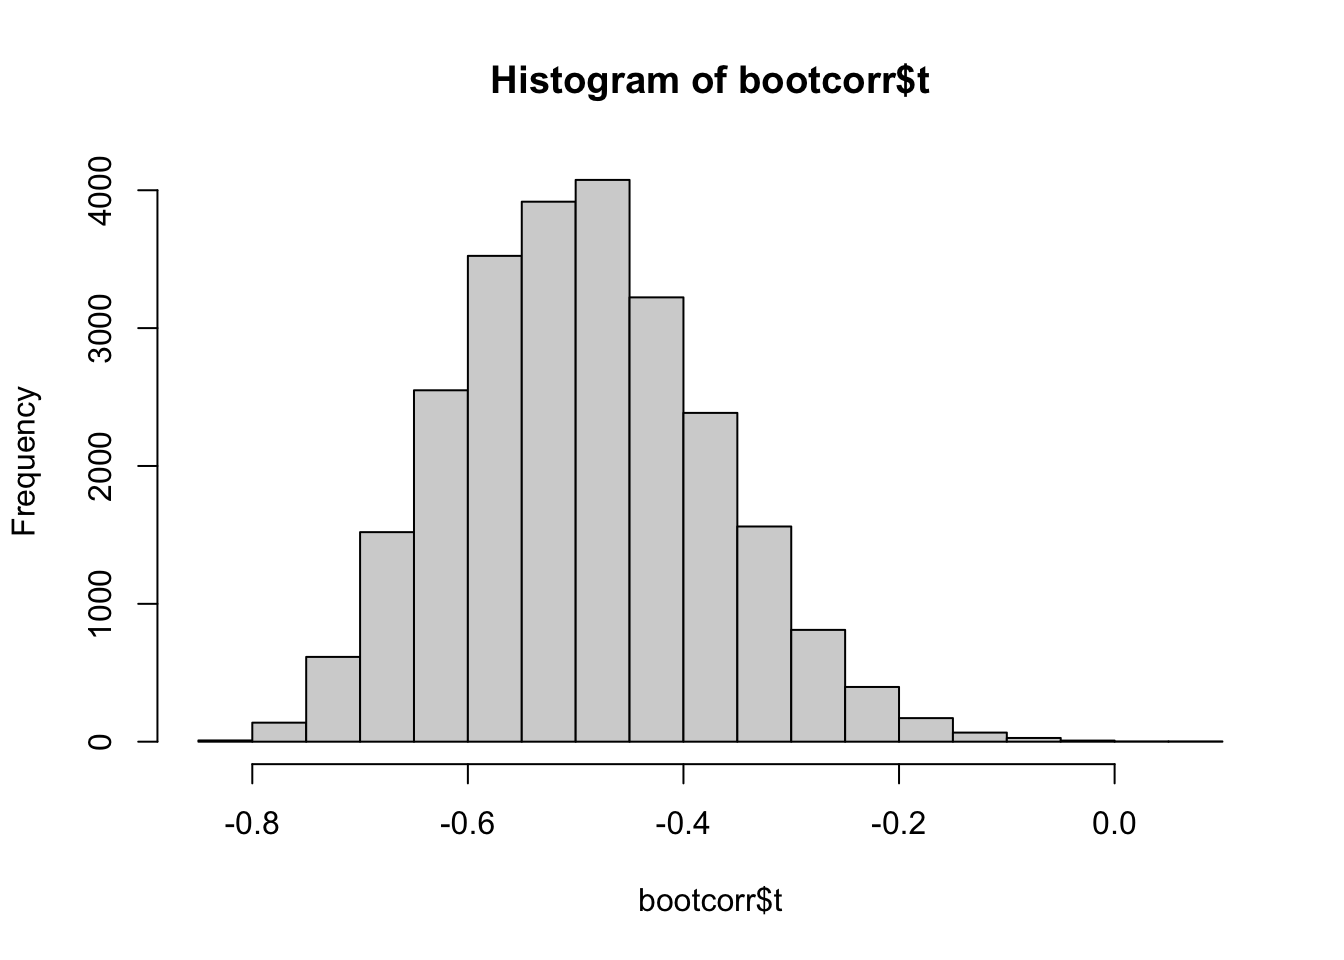
\includegraphics[keepaspectratio]{_main_files/figure-latex/boostrapexercise-1.pdf}}

\begin{Shaded}
\begin{Highlighting}[]
  \CommentTok{\#or }
  \CommentTok{\#hist(cor.boot)}
\end{Highlighting}
\end{Shaded}

\chapter{Cross-validation}\label{cross-validation}

\section{Introduction}\label{cv.intro}

When assessing the performance of a model in the same data that was used to
fit the model, we will be overestimating the model performance. A better
strategy is to initially split the data and use one part to fit the model and
the other one to test it. In machine learning terminology the data used to fit
the model is called the \textbf{training data} and the data used to assess the model
performance is called \textbf{testing data}.

The cross-validation is a repetition of the process above but each time we
use a different split of the data. This will result in several measures of
performance obtained in each split combination. The final performance
statistics is obtained by averaging all results of the different splits.

\section{Readings}\label{cv.read}

Read the following chapter of \emph{An introduction to statistical learning}:

\begin{itemize}
\tightlist
\item
  5.1 Cross-validation
\end{itemize}

\section{Practice session}\label{cv.prac}

\subsection*{\texorpdfstring{Task 1 - Cross-validated MSE and R\textsuperscript{2}}{Task 1 - Cross-validated MSE and R2}}\label{task-1---cross-validated-mse-and-r2}
\addcontentsline{toc}{subsection}{Task 1 - Cross-validated MSE and R\textsuperscript{2}}

We will be using the
\href{https://www.dropbox.com/s/7wjsfdaf0wt2kg2/bmd.csv?dl=1}{bmd.csv}
dataset to fit a linear model for \emph{bmd} using \emph{age}, \emph{sex} and \emph{bmi},
and compute the cross-validated MSE and \(R^2\).
We will fit the model with main effects using 10 times a 5-fold cross-validation.

We will use the tools from the \textbf{caret} package.
This is a powerful package that wraps several methods for regression and
classification: \href{http://topepo.github.io/caret/index.html}{manual}

\texttt{}

\begin{Shaded}
\begin{Highlighting}[]
\FunctionTok{library}\NormalTok{(e1071)}
\FunctionTok{library}\NormalTok{(caret) }\CommentTok{\#library for Machine Learning}
\FunctionTok{library}\NormalTok{(boot)  }\CommentTok{\#library for bootstrap}
\FunctionTok{library}\NormalTok{(pROC)  }\CommentTok{\#library for the ROC curve}
\FunctionTok{library}\NormalTok{(Rmisc) }\CommentTok{\#CI() function to compute the conf interval for the mean}
\FunctionTok{set.seed}\NormalTok{(}\DecValTok{1974}\NormalTok{)}
\CommentTok{\#the option stringsAsFactors = TRUE in the command below converts }
\CommentTok{\#string variables as sex into factor variables}
\NormalTok{bmd.data }\OtherTok{\textless{}{-}} \FunctionTok{read.csv}\NormalTok{(}\StringTok{"https://www.dropbox.com/s/c6mhgatkotuze8o/bmd.csv?dl=1"}\NormalTok{, }
                     \AttributeTok{stringsAsFactors =} \ConstantTok{TRUE}\NormalTok{)}
\CommentTok{\#computes the BMI}
\NormalTok{bmd.data}\SpecialCharTok{$}\NormalTok{bmi }\OtherTok{\textless{}{-}}\NormalTok{ bmd.data}\SpecialCharTok{$}\NormalTok{weight\_kg }\SpecialCharTok{/}\NormalTok{ (bmd.data}\SpecialCharTok{$}\NormalTok{height\_cm}\SpecialCharTok{/}\DecValTok{100}\NormalTok{)}\SpecialCharTok{\^{}}\DecValTok{2}
\end{Highlighting}
\end{Shaded}

\begin{Shaded}
\begin{Highlighting}[]
\NormalTok{trC.lm }\OtherTok{\textless{}{-}} \FunctionTok{trainControl}\NormalTok{(                  }\CommentTok{\#defines the CV procedure}
                 \AttributeTok{method =} \StringTok{"repeatedcv"}\NormalTok{,  }\CommentTok{\#multiple CV}
                 \AttributeTok{number =} \DecValTok{5}\NormalTok{,            }\CommentTok{\#5{-}fold CV}
                 \AttributeTok{repeats =} \DecValTok{10}\NormalTok{)          }\CommentTok{\#repeats the cross validation 10 times}

\CommentTok{\#fits the linear model with CV defined above}
\NormalTok{model.lm }\OtherTok{\textless{}{-}} \FunctionTok{train}\NormalTok{(bmd }\SpecialCharTok{\textasciitilde{}}\NormalTok{ age }\SpecialCharTok{+}\NormalTok{ sex }\SpecialCharTok{+}\NormalTok{ bmi, }
                \AttributeTok{data =}\NormalTok{ bmd.data, }
                \AttributeTok{method =} \StringTok{"lm"}\NormalTok{, }
                \AttributeTok{trControl =}\NormalTok{ trC.lm)}

\NormalTok{model.lm}
\end{Highlighting}
\end{Shaded}

\begin{verbatim}
## Linear Regression 
## 
## 169 samples
##   3 predictor
## 
## No pre-processing
## Resampling: Cross-Validated (5 fold, repeated 10 times) 
## Summary of sample sizes: 136, 135, 134, 135, 136, 136, ... 
## Resampling results:
## 
##   RMSE      Rsquared  MAE      
##   0.137992  0.331976  0.1044175
## 
## Tuning parameter 'intercept' was held constant at a value of TRUE
\end{verbatim}

\begin{Shaded}
\begin{Highlighting}[]
\FunctionTok{summary}\NormalTok{(model.lm}\SpecialCharTok{$}\NormalTok{finalModel)}
\end{Highlighting}
\end{Shaded}

\begin{verbatim}
## 
## Call:
## lm(formula = .outcome ~ ., data = dat)
## 
## Residuals:
##      Min       1Q   Median       3Q      Max 
## -0.38207 -0.07669 -0.00654  0.07888  0.51256 
## 
## Coefficients:
##               Estimate Std. Error t value Pr(>|t|)    
## (Intercept)  0.6063945  0.0834051   7.270 1.36e-11 ***
## age         -0.0041579  0.0008625  -4.821 3.23e-06 ***
## sexM         0.0949602  0.0213314   4.452 1.56e-05 ***
## bmi          0.0155913  0.0024239   6.432 1.30e-09 ***
## ---
## Signif. codes:  0 '***' 0.001 '**' 0.01 '*' 0.05 '.' 0.1 ' ' 1
## 
## Residual standard error: 0.138 on 165 degrees of freedom
## Multiple R-squared:  0.3254, Adjusted R-squared:  0.3131 
## F-statistic: 26.53 on 3 and 165 DF,  p-value: 4.677e-14
\end{verbatim}

\textbf{TRY IT YOURSELF:}

\begin{enumerate}
\def\labelenumi{\arabic{enumi})}
\tightlist
\item
  Refit the same model and evaluate the MSE and \(R^2\) using leave one out (\textbf{method = ``LOOCV''})
\end{enumerate}

\emph{See the solution code}

\begin{Shaded}
\begin{Highlighting}[]
\NormalTok{trC.lm.loocv }\OtherTok{\textless{}{-}} \FunctionTok{trainControl}\NormalTok{(  }
                 \AttributeTok{method =} \StringTok{"LOOCV"}\NormalTok{) }\CommentTok{\# leave on out CV}
                   
\NormalTok{model.lm2 }\OtherTok{\textless{}{-}} \FunctionTok{train}\NormalTok{(bmd }\SpecialCharTok{\textasciitilde{}}\NormalTok{ age }\SpecialCharTok{+}\NormalTok{ sex }\SpecialCharTok{+}\NormalTok{ bmi, }
                \AttributeTok{data =}\NormalTok{ bmd.data, }\AttributeTok{method =} \StringTok{"lm"}\NormalTok{,}
                \AttributeTok{trControl =}\NormalTok{ trC.lm.loocv)}

\NormalTok{model.lm2}
\FunctionTok{summary}\NormalTok{(model.lm2}\SpecialCharTok{$}\NormalTok{finalModel)}
\end{Highlighting}
\end{Shaded}

\begin{enumerate}
\def\labelenumi{\arabic{enumi})}
\setcounter{enumi}{1}
\tightlist
\item
  Fit a k nearest neighbour regression for BMD using AGE, SEX and BMI,
  and choose the k (number of neighbours) by 10-fold cross-validation
  repeated 10 times. Also, obtain the MSE and \(R^2\).
\end{enumerate}

NOTE1: you need the make sure all the predictors are in the same scale. You can
either use the '\texttt{scale()} function or add \texttt{preProcess\ =\ c("center","scale")} to
the \texttt{train()} function.

NOTE2: you can either use \texttt{tuneLength\ =\ 20} to define the number of neighbours
or \texttt{tuneGrid=expand.grid(k=seq(1,43,2))}

\emph{See the solution code}

\begin{Shaded}
\begin{Highlighting}[]
\NormalTok{trC.knn }\OtherTok{\textless{}{-}} \FunctionTok{trainControl}\NormalTok{(    }
                 \AttributeTok{method =} \StringTok{"repeatedcv"}\NormalTok{, }\CommentTok{\# multiple CV}
                 \AttributeTok{number =} \DecValTok{10}\NormalTok{,  }\CommentTok{\#10{-}fold CV}
                 \AttributeTok{repeats =} \DecValTok{10}\NormalTok{)}

\NormalTok{model.knn }\OtherTok{\textless{}{-}} \FunctionTok{train}\NormalTok{(bmd }\SpecialCharTok{\textasciitilde{}}\NormalTok{ age }\SpecialCharTok{+}\NormalTok{ sex }\SpecialCharTok{+}\NormalTok{ bmi, }
                \AttributeTok{data =}\NormalTok{ bmd.data, }\AttributeTok{method =} \StringTok{"knn"}\NormalTok{,}
                \AttributeTok{trControl =}\NormalTok{ trC.knn,}
                \AttributeTok{preProcess =} \FunctionTok{c}\NormalTok{(}\StringTok{"center"}\NormalTok{,}\StringTok{"scale"}\NormalTok{),}
                \AttributeTok{tuneLength =} \DecValTok{20}\NormalTok{)   }\CommentTok{\#instead of tuneLength, we could have}
                                  \CommentTok{\#used tuneGrid=expand.grid(k=1:40)}
\CommentTok{\# Model Summary}
\NormalTok{model.knn}
\NormalTok{model.knn}\SpecialCharTok{$}\NormalTok{results}

\CommentTok{\#results in each cv{-}fold}
\NormalTok{model.knn}\SpecialCharTok{$}\NormalTok{resample}
\FunctionTok{plot}\NormalTok{(model.knn)}
\end{Highlighting}
\end{Shaded}

\pandocbounded{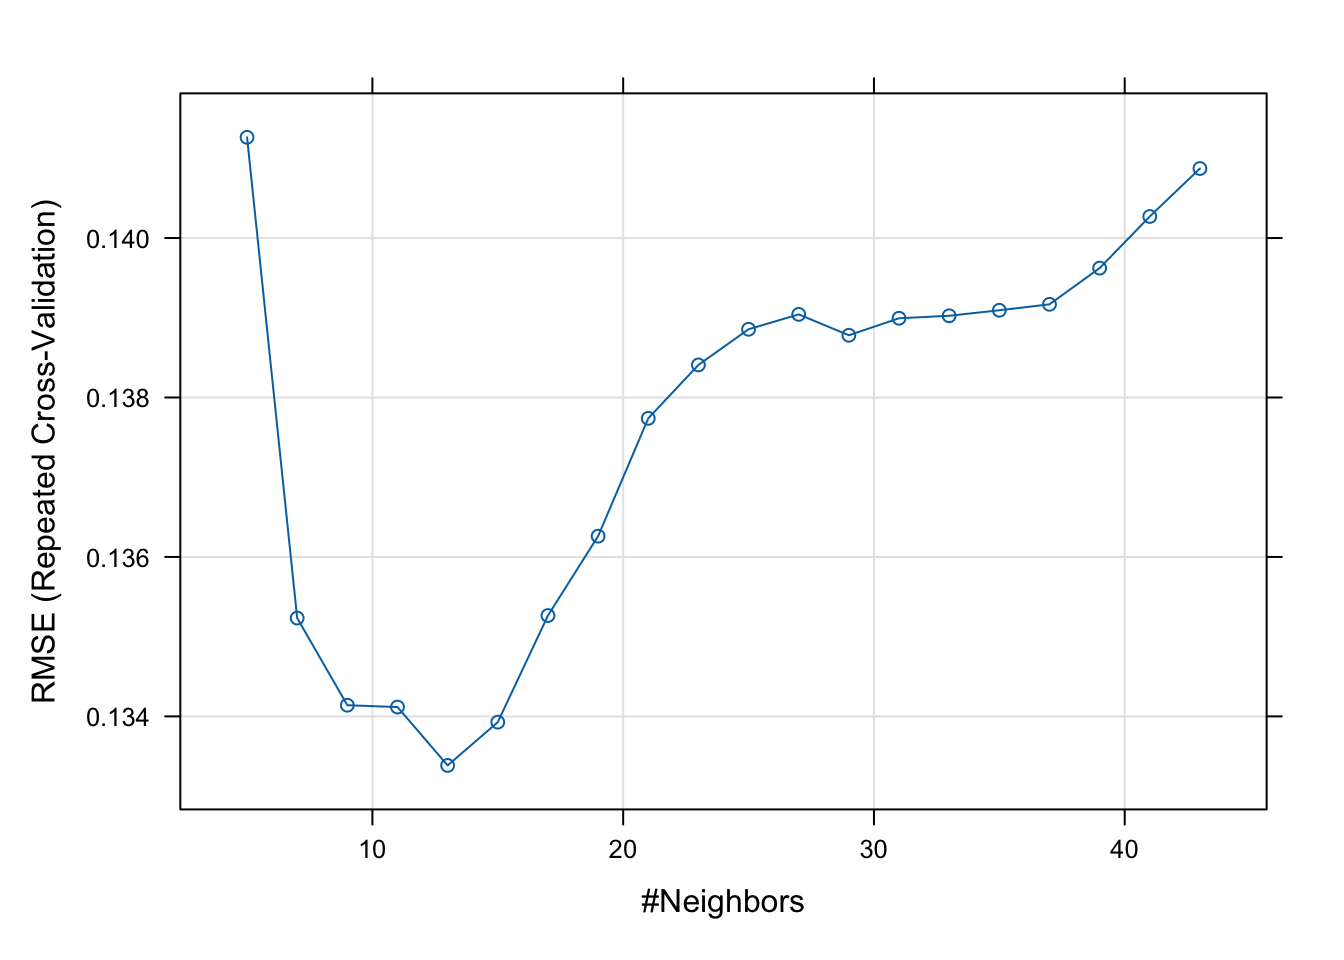
\includegraphics[keepaspectratio]{_main_files/figure-latex/unnamed-chunk-9-1.pdf}}

\subsection*{Task 2 - ROC cross-validation}\label{task-2---roc-cross-validation}
\addcontentsline{toc}{subsection}{Task 2 - ROC cross-validation}

We want to fit the following model \textbf{logit(fracture) \textasciitilde{} age + sex + bmi +bmd}
and assess its performance by computing the area under the ROC curve
using cross-validation

\begin{Shaded}
\begin{Highlighting}[]
\CommentTok{\#caret does not like the category "no fracture"}
\CommentTok{\#because of the space}
\CommentTok{\#We are creating a new label for the categories}
\NormalTok{bmd.data}\SpecialCharTok{$}\NormalTok{fract }\OtherTok{\textless{}{-}} \FunctionTok{ifelse}\NormalTok{ (bmd.data}\SpecialCharTok{$}\NormalTok{fracture }\SpecialCharTok{==}\StringTok{"fracture"}\NormalTok{, }\StringTok{"F"}\NormalTok{, }\StringTok{"NF"}\NormalTok{)}
\NormalTok{bmd.data}\SpecialCharTok{$}\NormalTok{fract }\OtherTok{\textless{}{-}} \FunctionTok{as.factor}\NormalTok{(bmd.data}\SpecialCharTok{$}\NormalTok{fract)}

\NormalTok{trC }\OtherTok{\textless{}{-}} \FunctionTok{trainControl}\NormalTok{(}
            \AttributeTok{method =} \StringTok{"cv"}\NormalTok{,     }\CommentTok{\#just 1 CV}
            \AttributeTok{number =} \DecValTok{10}\NormalTok{,       }\CommentTok{\#10{-}fold CV}
            \AttributeTok{classProbs =} \ConstantTok{TRUE}\NormalTok{,}
            \AttributeTok{summaryFunction =}\NormalTok{ twoClassSummary,}
            \AttributeTok{savePred =}\ConstantTok{TRUE}\NormalTok{)  }\CommentTok{\#to be used in the confusion matrix}

\NormalTok{model.LR }\OtherTok{\textless{}{-}} \FunctionTok{train}\NormalTok{(fract }\SpecialCharTok{\textasciitilde{}}\NormalTok{ age }\SpecialCharTok{+}\NormalTok{ sex }\SpecialCharTok{+}\NormalTok{ bmi }\SpecialCharTok{+}\NormalTok{ bmd , }
                \AttributeTok{data =}\NormalTok{ bmd.data, }\AttributeTok{method =} \StringTok{"glm"}\NormalTok{,}
                \AttributeTok{family=}\StringTok{"binomial"}\NormalTok{,}
                \AttributeTok{trControl =}\NormalTok{ trC,}
                \AttributeTok{metric =} \StringTok{"ROC"}\NormalTok{)}


\CommentTok{\# Model Summary}
\NormalTok{model.LR}
\end{Highlighting}
\end{Shaded}

\begin{verbatim}
## Generalized Linear Model 
## 
## 169 samples
##   4 predictor
##   2 classes: 'F', 'NF' 
## 
## No pre-processing
## Resampling: Cross-Validated (10 fold) 
## Summary of sample sizes: 152, 152, 152, 152, 152, 152, ... 
## Resampling results:
## 
##   ROC        Sens  Spec     
##   0.8980303  0.72  0.9166667
\end{verbatim}

\begin{Shaded}
\begin{Highlighting}[]
\NormalTok{model.LR}\SpecialCharTok{$}\NormalTok{results}
\end{Highlighting}
\end{Shaded}

\begin{verbatim}
##   parameter       ROC Sens      Spec     ROCSD    SensSD     SpecSD
## 1      none 0.8980303 0.72 0.9166667 0.1362458 0.1686548 0.09622504
\end{verbatim}

\begin{Shaded}
\begin{Highlighting}[]
\CommentTok{\#results in each cv{-}fold}
\NormalTok{model.LR}\SpecialCharTok{$}\NormalTok{resample}
\end{Highlighting}
\end{Shaded}

\begin{verbatim}
##          ROC Sens      Spec Resample
## 1  0.9500000  0.6 1.0000000   Fold01
## 2  0.7500000  0.6 0.9166667   Fold02
## 3  0.9666667  0.6 0.9166667   Fold03
## 4  0.9000000  0.8 1.0000000   Fold04
## 5  0.5666667  0.6 0.6666667   Fold05
## 6  0.9666667  1.0 0.9166667   Fold06
## 7  0.9636364  0.6 1.0000000   Fold07
## 8  0.9833333  0.8 0.9166667   Fold08
## 9  0.9333333  0.6 0.9166667   Fold09
## 10 1.0000000  1.0 0.9166667   Fold10
\end{verbatim}

\begin{Shaded}
\begin{Highlighting}[]
\CommentTok{\#Confusion matrix cross{-}validated}
\FunctionTok{confusionMatrix}\NormalTok{(model.LR)}
\end{Highlighting}
\end{Shaded}

\begin{verbatim}
## Cross-Validated (10 fold) Confusion Matrix 
## 
## (entries are percentual average cell counts across resamples)
##  
##           Reference
## Prediction    F   NF
##         F  21.3  5.9
##         NF  8.3 64.5
##                            
##  Accuracy (average) : 0.858
\end{verbatim}

\begin{Shaded}
\begin{Highlighting}[]
\CommentTok{\#Confusion matrix for the final model}
\NormalTok{pred.LR  }\OtherTok{\textless{}{-}} \FunctionTok{predict}\NormalTok{(model.LR)}
\FunctionTok{confusionMatrix}\NormalTok{(}\AttributeTok{data=}\NormalTok{pred.LR, }\AttributeTok{reference=}\NormalTok{bmd.data}\SpecialCharTok{$}\NormalTok{fract)}
\end{Highlighting}
\end{Shaded}

\begin{verbatim}
## Confusion Matrix and Statistics
## 
##           Reference
## Prediction   F  NF
##         F   35   9
##         NF  15 110
##                                           
##                Accuracy : 0.858           
##                  95% CI : (0.7961, 0.9068)
##     No Information Rate : 0.7041          
##     P-Value [Acc > NIR] : 2.272e-06       
##                                           
##                   Kappa : 0.6469          
##                                           
##  Mcnemar's Test P-Value : 0.3074          
##                                           
##             Sensitivity : 0.7000          
##             Specificity : 0.9244          
##          Pos Pred Value : 0.7955          
##          Neg Pred Value : 0.8800          
##              Prevalence : 0.2959          
##          Detection Rate : 0.2071          
##    Detection Prevalence : 0.2604          
##       Balanced Accuracy : 0.8122          
##                                           
##        'Positive' Class : F               
## 
\end{verbatim}

\textbf{TRY IT YOURSELF}

\begin{enumerate}
\def\labelenumi{\arabic{enumi})}
\tightlist
\item
  Use the KNN algorithm to predict \textbf{fracture} based on the same variables
  of the logistic model above, by choosing the \emph{k} using cross-validation and
  compute the area under the ROC.
\end{enumerate}

\emph{See the solution code}

\begin{Shaded}
\begin{Highlighting}[]
\NormalTok{trC.knn }\OtherTok{\textless{}{-}} \FunctionTok{trainControl}\NormalTok{(}
            \AttributeTok{method =} \StringTok{"cv"}\NormalTok{,     }\CommentTok{\#just 1 CV}
            \AttributeTok{number =} \DecValTok{10}\NormalTok{,       }\CommentTok{\#10{-}fold CV}
            \AttributeTok{classProbs =} \ConstantTok{TRUE}\NormalTok{,}
            \AttributeTok{summaryFunction =}\NormalTok{ twoClassSummary,}
            \AttributeTok{savePred =}\ConstantTok{TRUE}\NormalTok{)  }\CommentTok{\#to be used in the confusion matrix}

\NormalTok{model.knn }\OtherTok{\textless{}{-}} \FunctionTok{train}\NormalTok{(fract }\SpecialCharTok{\textasciitilde{}}\NormalTok{ age }\SpecialCharTok{+}\NormalTok{ sex }\SpecialCharTok{+}\NormalTok{ bmi }\SpecialCharTok{+}\NormalTok{ bmd , }
                \AttributeTok{data =}\NormalTok{ bmd.data, }\AttributeTok{method =} \StringTok{"knn"}\NormalTok{,}
                \AttributeTok{trControl =}\NormalTok{ trC.knn,}
                \AttributeTok{tuneLength =} \DecValTok{30}\NormalTok{,}
                \AttributeTok{preProcess =} \FunctionTok{c}\NormalTok{(}\StringTok{"center"}\NormalTok{,}\StringTok{"scale"}\NormalTok{),}
                \AttributeTok{metric =} \StringTok{"ROC"}\NormalTok{)}


\CommentTok{\# Model Summary}
\NormalTok{model.knn}
\FunctionTok{plot}\NormalTok{(model.knn)}
\end{Highlighting}
\end{Shaded}

\pandocbounded{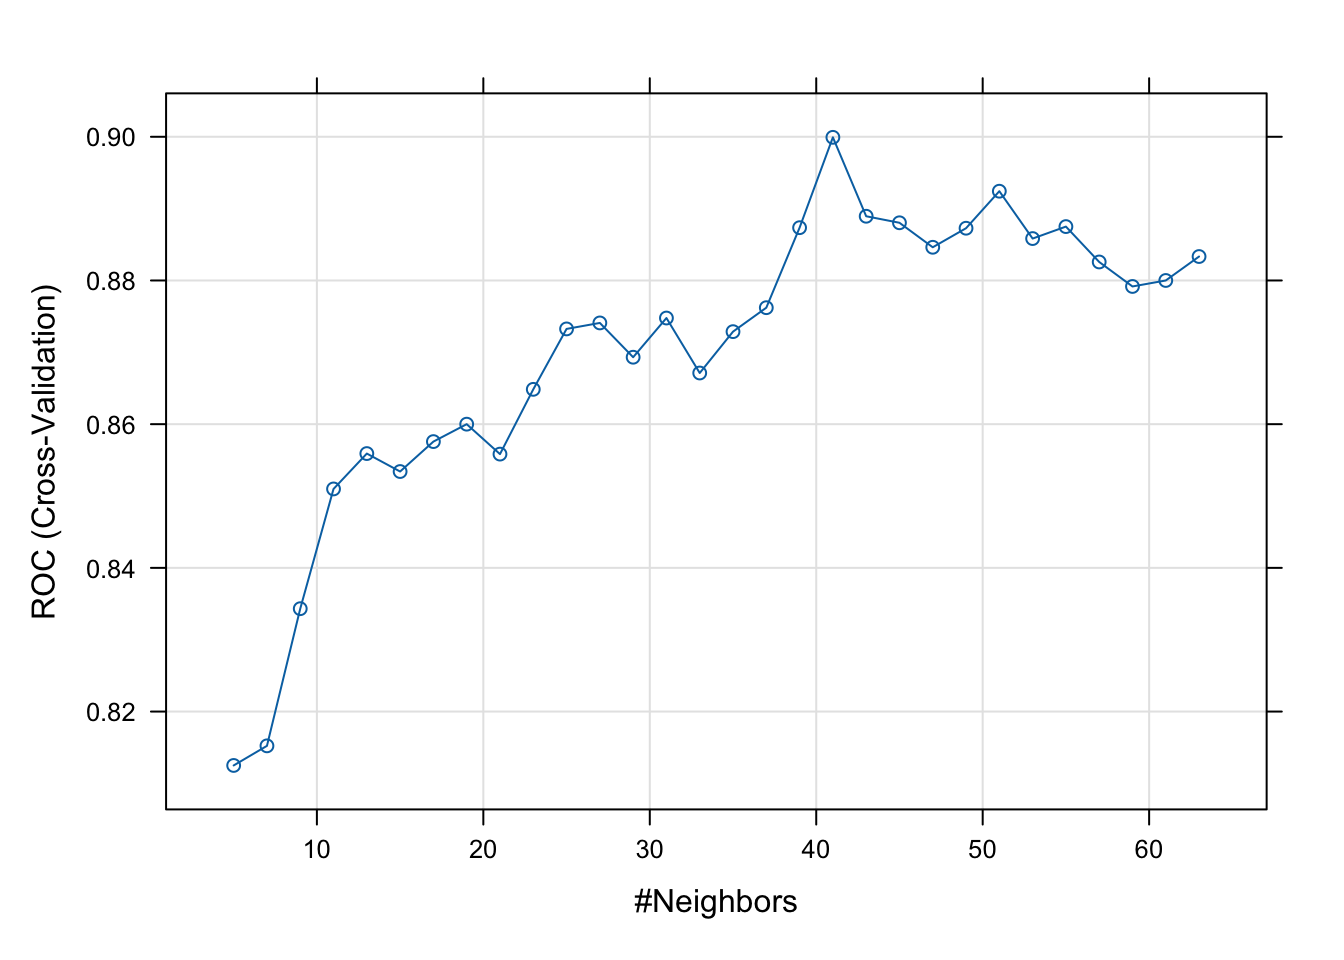
\includegraphics[keepaspectratio]{_main_files/figure-latex/unnamed-chunk-11-1.pdf}}

\begin{Shaded}
\begin{Highlighting}[]
\NormalTok{model.knn}\SpecialCharTok{$}\NormalTok{results}

\CommentTok{\#results in each cv{-}fold}
\NormalTok{model.knn}\SpecialCharTok{$}\NormalTok{resample}

\CommentTok{\#Confusion matrix cross{-}validated}
\FunctionTok{confusionMatrix}\NormalTok{(model.knn)}

\CommentTok{\#Confusion matrix for the final model}
\NormalTok{pred.knn  }\OtherTok{\textless{}{-}} \FunctionTok{predict}\NormalTok{(model.knn)}
\FunctionTok{confusionMatrix}\NormalTok{(}\AttributeTok{data=}\NormalTok{pred.knn, }\AttributeTok{reference=}\NormalTok{bmd.data}\SpecialCharTok{$}\NormalTok{fract)}
\end{Highlighting}
\end{Shaded}

\subsection*{Task 3 - Classification}\label{task-3---classification}
\addcontentsline{toc}{subsection}{Task 3 - Classification}

Read the dataset \href{https://www.dropbox.com/s/wg32uj43fsy9yvd/SBI.csv?dl=0}{SBI.csv}
and create a prediction model for the outcome ``sbi'' using ``age'', ``pct'', ``crp'',
``wcc'' and ``fever\_hours'' as predictors (you can read.

Let's first read the data in

\begin{Shaded}
\begin{Highlighting}[]
\NormalTok{sbi.data     }\OtherTok{\textless{}{-}} 
  \FunctionTok{read.csv}\NormalTok{(}\StringTok{"https://www.dropbox.com/s/wg32uj43fsy9yvd/SBI.csv?dl=1"}\NormalTok{, }
           \AttributeTok{stringsAsFactors =} \ConstantTok{TRUE}\NormalTok{)}
\FunctionTok{summary}\NormalTok{(sbi.data)}
\end{Highlighting}
\end{Shaded}

\begin{verbatim}
##        X                id          fever_hours           age        sex     
##  Min.   :   1.0   Min.   :   495   Min.   :   0.00   Min.   :0.010   F:1013  
##  1st Qu.: 587.8   1st Qu.:133039   1st Qu.:  24.00   1st Qu.:0.760   M:1335  
##  Median :1174.5   Median :160016   Median :  48.00   Median :1.525           
##  Mean   :1174.5   Mean   :153698   Mean   :  80.06   Mean   :1.836           
##  3rd Qu.:1761.2   3rd Qu.:196030   3rd Qu.:  78.00   3rd Qu.:2.752           
##  Max.   :2348.0   Max.   :229986   Max.   :3360.00   Max.   :4.990           
##       wcc          prevAB                sbi            pct           
##  Min.   : 0.2368   No :1370   Bact         :  34   Min.   :  0.00865  
##  1st Qu.: 7.9000   Yes: 978   NotApplicable:1752   1st Qu.:  0.16000  
##  Median :11.6000              Pneu         : 251   Median :  0.76000  
##  Mean   :12.6431              UTI          : 311   Mean   :  3.74354  
##  3rd Qu.:16.1000                                   3rd Qu.:  4.61995  
##  Max.   :58.7000                                   Max.   :156.47000  
##       crp        
##  Min.   :  0.00  
##  1st Qu.: 11.83  
##  Median : 30.97  
##  Mean   : 48.41  
##  3rd Qu.: 66.20  
##  Max.   :429.90
\end{verbatim}

We will try different approaches starting with linear discriminant analysis

\begin{Shaded}
\begin{Highlighting}[]
\NormalTok{trCtrl.lda }\OtherTok{\textless{}{-}} \FunctionTok{trainControl}\NormalTok{(}\AttributeTok{method =} \StringTok{"repeatedcv"}\NormalTok{,}
                           \AttributeTok{number =} \DecValTok{10}\NormalTok{,  }\CommentTok{\#10{-}fold CV}
                           \AttributeTok{repeats =} \DecValTok{10}\NormalTok{,}
                           \AttributeTok{classProbs =} \ConstantTok{TRUE}\NormalTok{,}
                           \AttributeTok{savePredictions =} \ConstantTok{TRUE}\NormalTok{)}
\NormalTok{model.lda }\OtherTok{\textless{}{-}} \FunctionTok{train}\NormalTok{(sbi }\SpecialCharTok{\textasciitilde{}}\NormalTok{ crp}\SpecialCharTok{+}\NormalTok{pct}\SpecialCharTok{+}\NormalTok{age}\SpecialCharTok{+}\NormalTok{wcc}\SpecialCharTok{+}\NormalTok{fever\_hours, }
                   \AttributeTok{data=}\NormalTok{sbi.data, }
                   \AttributeTok{method=}\StringTok{"lda"}\NormalTok{,}
                   \AttributeTok{trControl =}\NormalTok{ trCtrl.lda,}
                   \AttributeTok{metric=}\StringTok{"Accuracy"}\NormalTok{ )}

\NormalTok{model.lda}\SpecialCharTok{$}\NormalTok{results}
\end{Highlighting}
\end{Shaded}

\begin{verbatim}
##   parameter  Accuracy      Kappa AccuracySD    KappaSD
## 1      none 0.7478769 0.09311667 0.01071987 0.04376718
\end{verbatim}

\begin{Shaded}
\begin{Highlighting}[]
\FunctionTok{confusionMatrix}\NormalTok{(}\FunctionTok{predict}\NormalTok{(model.lda), sbi.data}\SpecialCharTok{$}\NormalTok{sbi)}
\end{Highlighting}
\end{Shaded}

\begin{verbatim}
## Confusion Matrix and Statistics
## 
##                Reference
## Prediction      Bact NotApplicable Pneu  UTI
##   Bact             5             5    7    6
##   NotApplicable   28          1722  238  273
##   Pneu             0             3    2    1
##   UTI              1            22    4   31
## 
## Overall Statistics
##                                          
##                Accuracy : 0.7496         
##                  95% CI : (0.7315, 0.767)
##     No Information Rate : 0.7462         
##     P-Value [Acc > NIR] : 0.3623         
##                                          
##                   Kappa : 0.0985         
##                                          
##  Mcnemar's Test P-Value : <2e-16         
## 
## Statistics by Class:
## 
##                      Class: Bact Class: NotApplicable Class: Pneu Class: UTI
## Sensitivity             0.147059              0.98288   0.0079681    0.09968
## Specificity             0.992221              0.09564   0.9980925    0.98675
## Pos Pred Value          0.217391              0.76161   0.3333333    0.53448
## Neg Pred Value          0.987527              0.65517   0.8936806    0.87773
## Prevalence              0.014480              0.74617   0.1068995    0.13245
## Detection Rate          0.002129              0.73339   0.0008518    0.01320
## Detection Prevalence    0.009796              0.96295   0.0025554    0.02470
## Balanced Accuracy       0.569640              0.53926   0.5030303    0.54321
\end{verbatim}

Now, let's try the logistic regression

\begin{Shaded}
\begin{Highlighting}[]
\NormalTok{trCtrl.lr }\OtherTok{\textless{}{-}} \FunctionTok{trainControl}\NormalTok{(}\AttributeTok{method =} \StringTok{"repeatedcv"}\NormalTok{,}
                           \AttributeTok{number =} \DecValTok{10}\NormalTok{,  }\CommentTok{\#10{-}fold CV}
                           \AttributeTok{repeats =} \DecValTok{10}\NormalTok{,}
                           \AttributeTok{classProbs =} \ConstantTok{TRUE}\NormalTok{,}
                           \AttributeTok{savePredictions =} \ConstantTok{TRUE}\NormalTok{)}
\NormalTok{model.lr }\OtherTok{\textless{}{-}} \FunctionTok{train}\NormalTok{(sbi }\SpecialCharTok{\textasciitilde{}}\NormalTok{ crp}\SpecialCharTok{+}\NormalTok{pct}\SpecialCharTok{+}\NormalTok{age}\SpecialCharTok{+}\NormalTok{wcc}\SpecialCharTok{+}\NormalTok{fever\_hours, }
                   \AttributeTok{data=}\NormalTok{sbi.data, }
                   \AttributeTok{method=}\StringTok{"multinom"}\NormalTok{,}
                   \AttributeTok{trControl =}\NormalTok{ trCtrl.lr,}
                   \AttributeTok{tuneLength=}\DecValTok{1}\NormalTok{)}
\end{Highlighting}
\end{Shaded}

\begin{Shaded}
\begin{Highlighting}[]
\NormalTok{model.lr}\SpecialCharTok{$}\NormalTok{results}
\end{Highlighting}
\end{Shaded}

\begin{verbatim}
##   decay  Accuracy      Kappa  AccuracySD    KappaSD
## 1     0 0.7516195 0.09927548 0.008932933 0.04049479
\end{verbatim}

\begin{Shaded}
\begin{Highlighting}[]
\FunctionTok{confusionMatrix}\NormalTok{(}\FunctionTok{predict}\NormalTok{(model.lr), sbi.data}\SpecialCharTok{$}\NormalTok{sbi)}
\end{Highlighting}
\end{Shaded}

\begin{verbatim}
## Confusion Matrix and Statistics
## 
##                Reference
## Prediction      Bact NotApplicable Pneu  UTI
##   Bact             0             1    1    0
##   NotApplicable   27          1727  241  270
##   Pneu             1             2    2    4
##   UTI              6            22    7   37
## 
## Overall Statistics
##                                           
##                Accuracy : 0.7521          
##                  95% CI : (0.7341, 0.7695)
##     No Information Rate : 0.7462          
##     P-Value [Acc > NIR] : 0.2618          
##                                           
##                   Kappa : 0.101           
##                                           
##  Mcnemar's Test P-Value : <2e-16          
## 
## Statistics by Class:
## 
##                      Class: Bact Class: NotApplicable Class: Pneu Class: UTI
## Sensitivity            0.0000000              0.98573   0.0079681    0.11897
## Specificity            0.9991357              0.09732   0.9966619    0.98282
## Pos Pred Value         0.0000000              0.76247   0.2222222    0.51389
## Neg Pred Value         0.9855072              0.69880   0.8935442    0.87961
## Prevalence             0.0144804              0.74617   0.1068995    0.13245
## Detection Rate         0.0000000              0.73552   0.0008518    0.01576
## Detection Prevalence   0.0008518              0.96465   0.0038330    0.03066
## Balanced Accuracy      0.4995678              0.54152   0.5023150    0.55089
\end{verbatim}

And finally, knn.

\begin{Shaded}
\begin{Highlighting}[]
\NormalTok{trCtrl.knn }\OtherTok{\textless{}{-}} \FunctionTok{trainControl}\NormalTok{(}\AttributeTok{method =} \StringTok{"repeatedcv"}\NormalTok{,}
                           \AttributeTok{number =} \DecValTok{10}\NormalTok{,  }\CommentTok{\#10{-}fold CV}
                           \AttributeTok{repeats =} \DecValTok{10}\NormalTok{,}
                           \AttributeTok{classProbs =} \ConstantTok{TRUE}\NormalTok{,}
                           \AttributeTok{savePredictions =} \ConstantTok{TRUE}\NormalTok{)}
\NormalTok{model.knn }\OtherTok{\textless{}{-}} \FunctionTok{train}\NormalTok{(sbi }\SpecialCharTok{\textasciitilde{}}\NormalTok{ crp}\SpecialCharTok{+}\NormalTok{pct}\SpecialCharTok{+}\NormalTok{age}\SpecialCharTok{+}\NormalTok{wcc}\SpecialCharTok{+}\NormalTok{fever\_hours, }
                   \AttributeTok{data=}\NormalTok{sbi.data, }
                   \AttributeTok{method=}\StringTok{"knn"}\NormalTok{,}
                   \AttributeTok{trControl =}\NormalTok{ trCtrl.knn,}
                   \AttributeTok{preProcess =} \FunctionTok{c}\NormalTok{(}\StringTok{"center"}\NormalTok{,}\StringTok{"scale"}\NormalTok{),}
                   \AttributeTok{tuneLength=}\DecValTok{20}\NormalTok{)}

\FunctionTok{plot}\NormalTok{(model.knn)}
\end{Highlighting}
\end{Shaded}

\pandocbounded{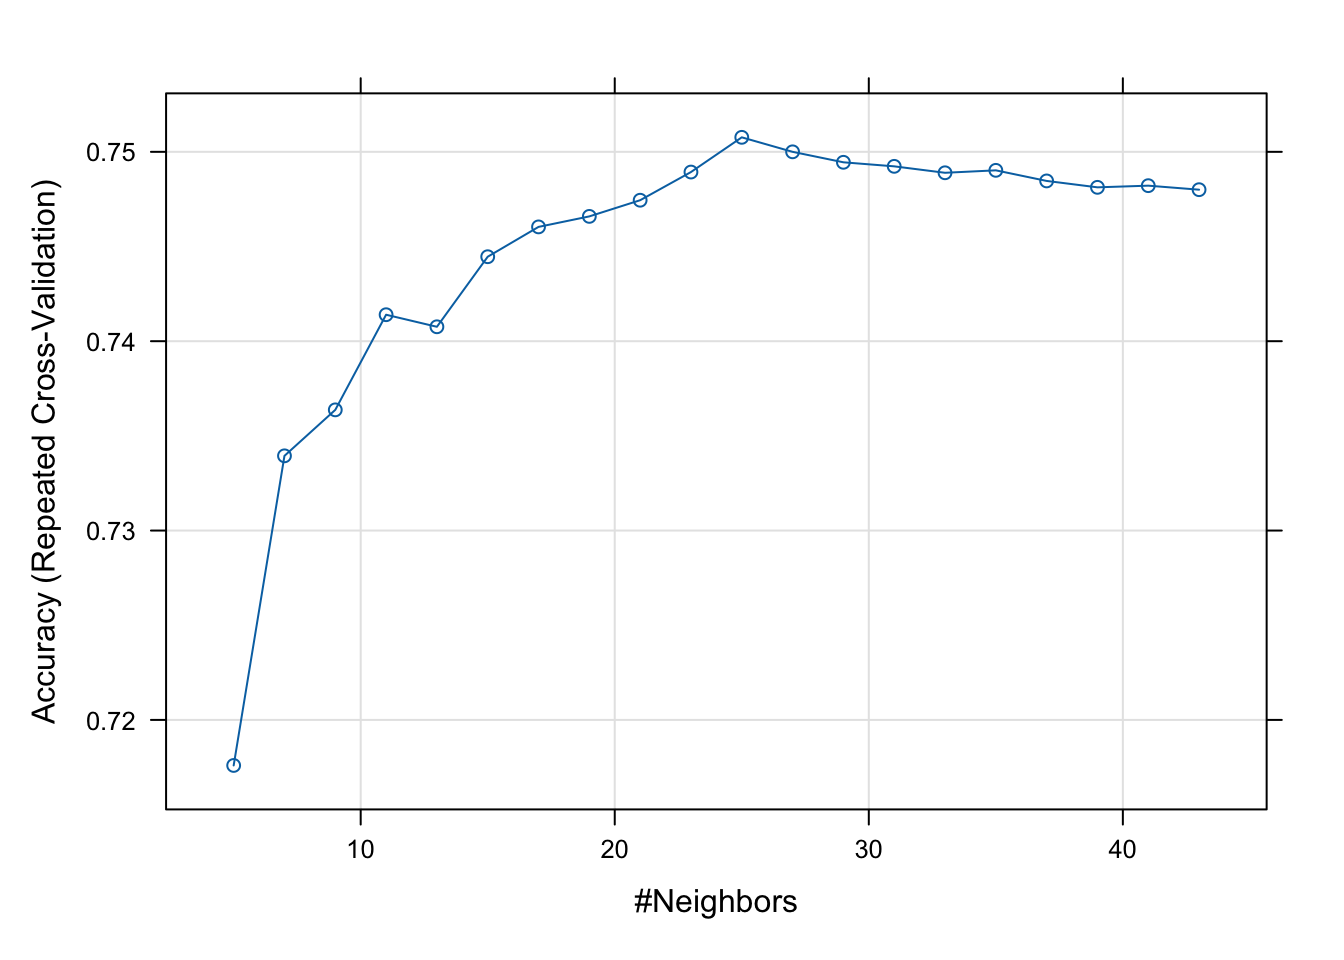
\includegraphics[keepaspectratio]{_main_files/figure-latex/unnamed-chunk-16-1.pdf}}

\begin{Shaded}
\begin{Highlighting}[]
\NormalTok{model.knn}
\end{Highlighting}
\end{Shaded}

\begin{verbatim}
## k-Nearest Neighbors 
## 
## 2348 samples
##    5 predictor
##    4 classes: 'Bact', 'NotApplicable', 'Pneu', 'UTI' 
## 
## Pre-processing: centered (5), scaled (5) 
## Resampling: Cross-Validated (10 fold, repeated 10 times) 
## Summary of sample sizes: 2114, 2114, 2113, 2114, 2113, 2112, ... 
## Resampling results across tuning parameters:
## 
##   k   Accuracy   Kappa     
##    5  0.7175953  0.12171412
##    7  0.7339458  0.12278852
##    9  0.7363738  0.10479303
##   11  0.7413980  0.10979312
##   13  0.7407610  0.09426706
##   15  0.7444609  0.09148660
##   17  0.7460360  0.08657437
##   19  0.7465912  0.08561247
##   21  0.7474448  0.08364397
##   23  0.7489325  0.08502779
##   25  0.7507663  0.08610948
##   27  0.7500005  0.07935699
##   29  0.7494477  0.07417419
##   31  0.7492342  0.07113888
##   33  0.7488938  0.06312317
##   35  0.7490229  0.05901425
##   37  0.7484635  0.05259630
##   39  0.7481255  0.04619287
##   41  0.7482135  0.04377731
##   43  0.7480011  0.04061429
## 
## Accuracy was used to select the optimal model using the largest value.
## The final value used for the model was k = 25.
\end{verbatim}

\begin{Shaded}
\begin{Highlighting}[]
\FunctionTok{confusionMatrix}\NormalTok{(}\FunctionTok{predict}\NormalTok{(model.knn), sbi.data}\SpecialCharTok{$}\NormalTok{sbi)}
\end{Highlighting}
\end{Shaded}

\begin{verbatim}
## Confusion Matrix and Statistics
## 
##                Reference
## Prediction      Bact NotApplicable Pneu  UTI
##   Bact             0             1    0    0
##   NotApplicable   29          1727  244  264
##   Pneu             0             1    2    1
##   UTI              5            23    5   46
## 
## Overall Statistics
##                                           
##                Accuracy : 0.756           
##                  95% CI : (0.7381, 0.7732)
##     No Information Rate : 0.7462          
##     P-Value [Acc > NIR] : 0.1429          
##                                           
##                   Kappa : 0.1154          
##                                           
##  Mcnemar's Test P-Value : NA              
## 
## Statistics by Class:
## 
##                      Class: Bact Class: NotApplicable Class: Pneu Class: UTI
## Sensitivity            0.0000000              0.98573   0.0079681    0.14791
## Specificity            0.9995678              0.09899   0.9990463    0.98380
## Pos Pred Value         0.0000000              0.76281   0.5000000    0.58228
## Neg Pred Value         0.9855134              0.70238   0.8937713    0.88321
## Prevalence             0.0144804              0.74617   0.1068995    0.13245
## Detection Rate         0.0000000              0.73552   0.0008518    0.01959
## Detection Prevalence   0.0004259              0.96422   0.0017036    0.03365
## Balanced Accuracy      0.4997839              0.54236   0.5035072    0.56585
\end{verbatim}

\section{Exercises}\label{cv.exerc}

\begin{enumerate}
\def\labelenumi{\arabic{enumi})}
\tightlist
\item
  What are the advantages and disadvantages of k-fold cross-
  validation relative to the validation set approach? And LOOCV?
\end{enumerate}

\emph{See the solution}

\emph{The validation set approach is conceptually simple and easily implemented as you are simply partitioning the existing training data into two sets. However, there are two drawbacks: (1.) the estimate of the test error rate can be highly variable depending on which observations are included in the training and validation sets. (2.) the validation set error rate may tend to overestimate the test error rate for the model fit on the entire data set.}

\emph{LOOCV is a special case of k-fold cross-validation with k = n.~Thus, LOOCV is the most computationally intense method since the model must be fit n times. Also, LOOCV has higher variance, but lower bias, than k-fold CV.}

\begin{enumerate}
\def\labelenumi{\arabic{enumi})}
\setcounter{enumi}{1}
\tightlist
\item
  Load the dataset \emph{PimaIndiansDiabetes} in the package \emph{mlbench} (you might need
  to install this package). This dataset consists of 768 observations
  of 9 variables: 8 variables which will be used as model
  predictors (number of times pregnant, plasma glucose concentration, diastolic blood pressure (mm Hg), triceps skin fold thickness (in mm), 2-hr serum insulin measure, body mass index, a diabetes pedigree function, and age) and 1 outcome variable (whether or not the patient has diabetes).\\
  Use the KNN algorithm to predict diabetes using all the predictors available.
  Choose the number of neighbours using cross-validation
\end{enumerate}

\emph{See the solution code}

\begin{Shaded}
\begin{Highlighting}[]
\CommentTok{\#install.packages("mlbench")}
\FunctionTok{library}\NormalTok{(mlbench)}
\FunctionTok{library}\NormalTok{(caret)}
\FunctionTok{library}\NormalTok{(class)}
\FunctionTok{set.seed}\NormalTok{(}\DecValTok{1999}\NormalTok{)}

\FunctionTok{data}\NormalTok{(PimaIndiansDiabetes)}


\NormalTok{trCtrl.knn.diab }\OtherTok{\textless{}{-}} \FunctionTok{trainControl}\NormalTok{(}\AttributeTok{method =} \StringTok{"repeatedcv"}\NormalTok{,}
                           \AttributeTok{number =} \DecValTok{10}\NormalTok{,  }\CommentTok{\#10{-}fold CV}
                           \AttributeTok{repeats =} \DecValTok{10}\NormalTok{,}
                           \AttributeTok{classProbs =} \ConstantTok{TRUE}\NormalTok{,}
                           \AttributeTok{savePredictions =} \ConstantTok{TRUE}\NormalTok{)}

\NormalTok{model.knn.diab  }\OtherTok{\textless{}{-}} \FunctionTok{train}\NormalTok{(diabetes }\SpecialCharTok{\textasciitilde{}}\NormalTok{ ., }
                   \AttributeTok{data =}\NormalTok{ PimaIndiansDiabetes, }
                   \AttributeTok{method=}\StringTok{"knn"}\NormalTok{,}
                   \AttributeTok{trControl =}\NormalTok{ trCtrl.knn.diab,}
                   \AttributeTok{tuneLength=}\DecValTok{20}\NormalTok{,}
                   \AttributeTok{preProcess =} \FunctionTok{c}\NormalTok{(}\StringTok{"center"}\NormalTok{,}\StringTok{"scale"}\NormalTok{))}
\NormalTok{model.knn.diab}
\end{Highlighting}
\end{Shaded}

\begin{verbatim}
## k-Nearest Neighbors 
## 
## 768 samples
##   8 predictor
##   2 classes: 'neg', 'pos' 
## 
## Pre-processing: centered (8), scaled (8) 
## Resampling: Cross-Validated (10 fold, repeated 10 times) 
## Summary of sample sizes: 691, 691, 691, 691, 691, 692, ... 
## Resampling results across tuning parameters:
## 
##   k   Accuracy   Kappa    
##    5  0.7389029  0.4053295
##    7  0.7394224  0.4047962
##    9  0.7468267  0.4180659
##   11  0.7434604  0.4096912
##   13  0.7364081  0.3904171
##   15  0.7416251  0.3977650
##   17  0.7485424  0.4127157
##   19  0.7541388  0.4228489
##   21  0.7557040  0.4227617
##   23  0.7588295  0.4297422
##   25  0.7515396  0.4093277
##   27  0.7471087  0.3962969
##   29  0.7489388  0.3985084
##   31  0.7505024  0.4013708
##   33  0.7534979  0.4066469
##   35  0.7541490  0.4071122
##   37  0.7521787  0.4003432
##   39  0.7513807  0.3975556
##   41  0.7530776  0.3995618
##   43  0.7523086  0.3964125
## 
## Accuracy was used to select the optimal model using the largest value.
## The final value used for the model was k = 23.
\end{verbatim}

\begin{Shaded}
\begin{Highlighting}[]
\FunctionTok{plot}\NormalTok{(model.knn.diab)}
\end{Highlighting}
\end{Shaded}

\pandocbounded{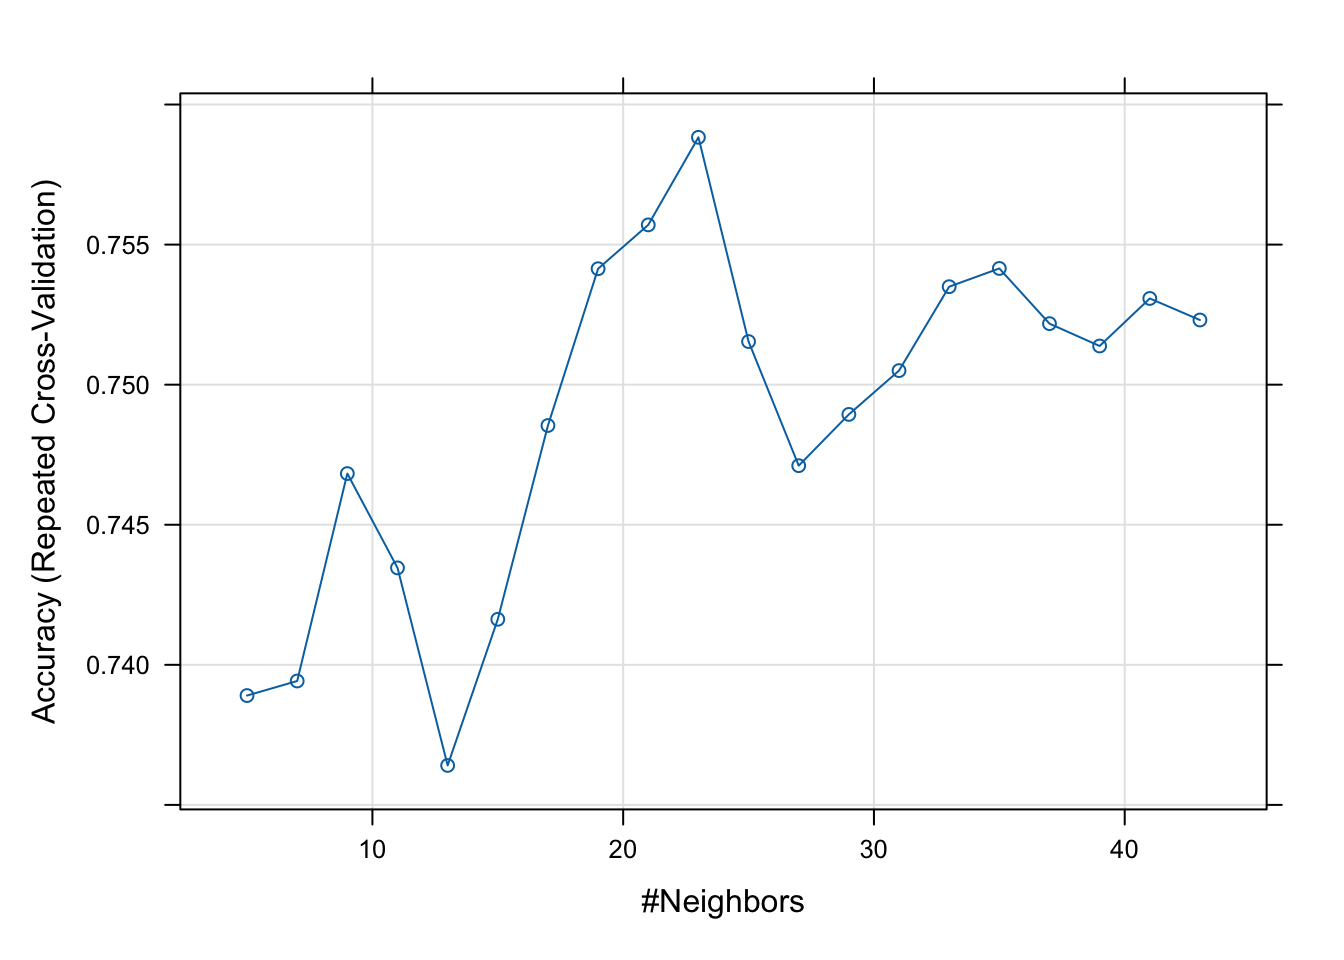
\includegraphics[keepaspectratio]{_main_files/figure-latex/unnamed-chunk-17-1.pdf}}

\end{document}
